\documentclass{standalone}
%\usepackage{import}
%\subimport{.../}{preamble}
\usepackage{tikz, graphicx, cmbright}
\begin{document}
\fontsize{10pt}{1em}\selectfont

\begin{tikzpicture}
\node [above right] at (0, 0) {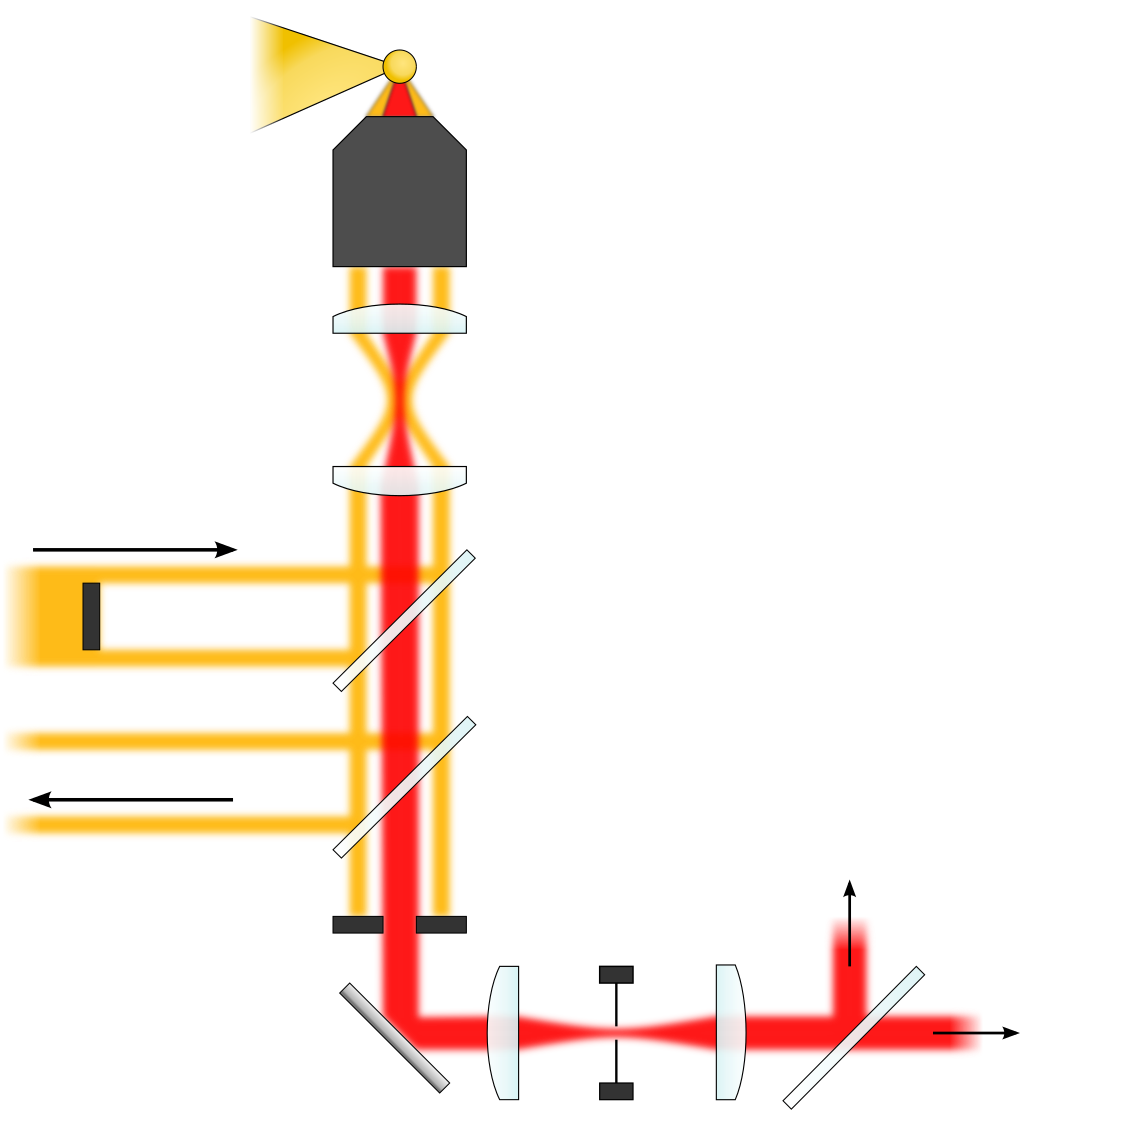
\includegraphics{simple_optics_layout.png}};
{\fontsize{9pt}{1em}\selectfont
{\color{white} \node [align=center] at (3.5, 8) {$100\times$\,IR\\obj.};}}
\node [align=center] at (1.6, 8.5) {$xyz$\\nanopositioning};
\node at (2.3, 6.3) {reimaging};
\node [align=left] at (1.5, 5.5) {supercontinuum\\illumination};
\node at (1.4, 3.1) {to CCD};
\node [align=center] at (5.4, 1.9) {confocal\\pinhole};
\node [align=center] at (7.4, 2.6) {transverse\\polarisation};
\node [align=center] at (8.9, 1.5) {axial\\polarisation};
\end{tikzpicture}

\end{document}